\documentclass[twocolumn]{revtex4}
\usepackage{graphics,graphicx,epsfig,ulem} 
\usepackage{amsmath}
\usepackage{multirow}
\usepackage{gensymb}
\usepackage{commath}
\usepackage{textcomp}
\newcommand{\squeezeup}{\vspace{-2.5mm}}

\begin{document}

\textheight=26.385cm
%Change textheight as the last resort...

\title{Determining the viscosity of water} 
 
 
\author{Jacky Cao, Room 205, Friday, Lab Partners: Peter Dorey, Jon Pritchett \\ Date of experiment: 11/11/2016, Date of report: 20/11/2016}


\begin{abstract}              
 
The volume flow rate of a fluid can be expressed functionally as derived by Poiseuille and Hagen. This relationship can be rearranged so that the viscosity of water can be experimentally determined. The volume and mass of water which has flowed out of a capillary tube for various heights can be measured. It is then possible to calculate a value for the viscosity. The average value obtained was determined to be $1.00 \pm 0.03$ mPa s, which does not agree with the literature value, $1.679$ mPa s \cite{crc}. 

\end{abstract}

\maketitle

\section{Introduction} 
\vspace{-2ex} 

Derived experimentally by Poiseuille in 1838 and Hagen in 1839 \cite{poiseuillehagen}, the volume flow rate $dV/dt$ of a fluid passing through a tube can be expressed as a function of the density of the fluid $\rho$, the value for acceleration due to gravity $g$, the height the fluid leaves the tube $h$, the radius $a$ and length $L$ of the tube, and the viscosity of the fluid $\eta$,

\squeezeup

\begin{equation} 
\frac{dV}{dt}=\frac{\pi}{8}\frac{\rho gh}{\eta}\frac{a^4}{L}. 
\label{pohagen}
\end{equation}

Noting that the group $\rho gh$ can be collectively termed as the pressure difference $\Delta P$ between the two ends of the tube \cite{collegephysics}. 

If we consider that a fluid is flowing through a tube like this, it experiences both friction with the inner wall and internal friction within itself. The latter can be defined more readily as the viscosity of the fluid $\eta$, and this results in shear stress when two adjacent layers (laminas) of fluid move relative to each other. 

We find that as $\eta$ increases, the volume flow rate decreases, the shear stress between two laminas becomes greater and so restricts the movement of the fluid's molecules trying to flow through the tube. 

Generally we can say that the lamina flow streamlines are smooth, the top layers of fluid are sliding over other laminas without the system having any turbulent motion - this condition is required for equation (\ref{pohagen}) to be valid. 

Using a rearranged form of the relation derived by Hagen and Poiseuille, and making initial assumptions, it is possible to experimentally calculate a value for the viscosity of water. Our assumptions being that the fluid is incompressible, the temperature of the water does not change, and the volume flow rate of water follows a linear relationship with height.

\vspace{-3ex}
\section{Method} 
\vspace{-2ex}
A flow of water was created by fixing a capillary tube to a water tank. The tank was raised to an initial height using an adjustable platform. The tank was then filled up with water from heights ($h$) 2cm to 16cm at 2cm intervals, these values were measured with the markings on the side of the tank. During this we had to ensure that we did not create parallax between the level of the water and the markings on the side. 

Water was allowed to flow out of the tube for a period of 90s for each height of water, this time was measured using a digital stopwatch. As the water flowed out it was caught within a large beaker so that the mass and volume of it could be measured after the allotted time had passed. 

The mass was found by having the beaker already on a set of electronic scales and initially zeroed to account for the beaker's mass. The volume on the other hand required the water to be transferred from the beaker to a measuring cylinder, this was performed by using a pipette. Care was again taken so that there was no parallax and that no unaccounted water was left within the beaker. It was also necessary to clear the tube once air bubbles formed along the length of it - this was done using a long piece of copper wire. 

\begin{figure}[!h]
\begin{center}
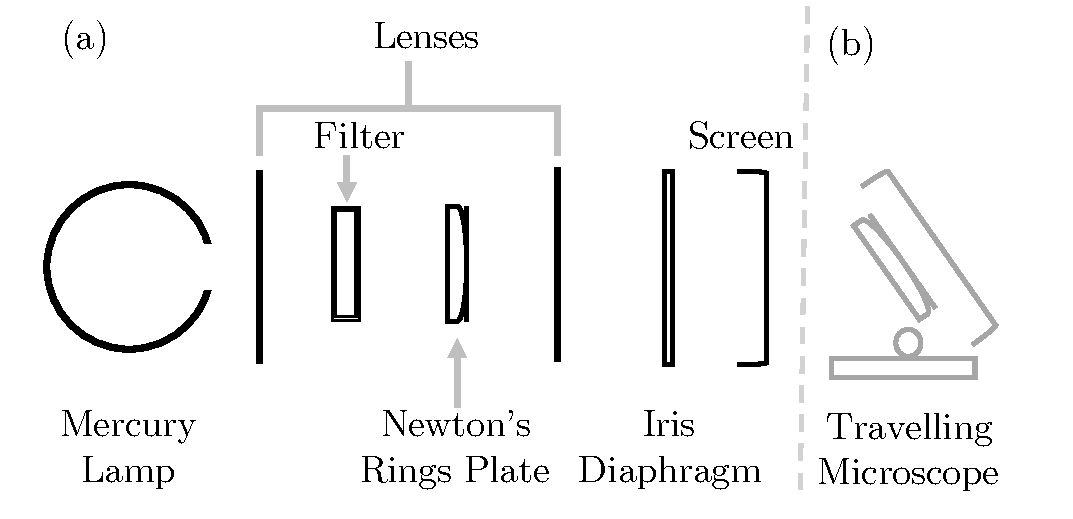
\includegraphics[width=5.7cm]{fig1}
\caption[]{A schematic of the experimental set-up used to collect data. }
\label{fig:fig1}
\end{center}
\end{figure}

\squeezeup
\squeezeup

An initial value for the density of water was calculated by taking four separate measurements of the volume and mass of the water, then calculating four individual values for $\rho_{water}$, and then averaging them.

One set of data was taken for each of the three capillary tubes that were used. Each tube varied in their internal diameter, $d$, this was measured using a travelling microscope along the horizontal axis. 

The collected data was applied to a least squares fitting to create an initial linear model.This was then used to calculate the flow rate for each different height, and thus allowing us to work out $\eta$.

\vspace{-3ex}
\section{Results}
\vspace{-2ex}

The volumetric flow rate of water is plotted against the varying height, as shown in Fig. \ref{fig:fig2}. This flow rate was calculated by dividing each value of the measured volume with the measured time period. Using this data, a value of viscosity could be calculated through a rearranged form of equation (\ref{pohagen}),

\squeezeup

\begin{equation} 
\eta=\frac{\pi \rho g a^4 }{8 L m}, 
\label{r-pohagen}
\end{equation}

where $m$ is the gradient of the least squares regression line, calculated with the known data for $dV/dt$ and $h$.

From preliminary results taking and analysis, our density of water is ${1001 \pm 1}$ kgm$^{-3}$.

The calculated values for the viscosity of water are shown in Table \ref{table:1} with which respective tube was used, the radius (found by dividing $d$ by two), and the reduced $\chi^2$ statistic for each of those tubes. 

An average value for viscosity can thus be found to be $1.00 \pm 0.03$ mPa s, which does not agree with the literature value \cite{crc}, $1.679$  mPa {s}. 

\vspace{-1ex}
\begin{figure}[!h]
\begin{center}
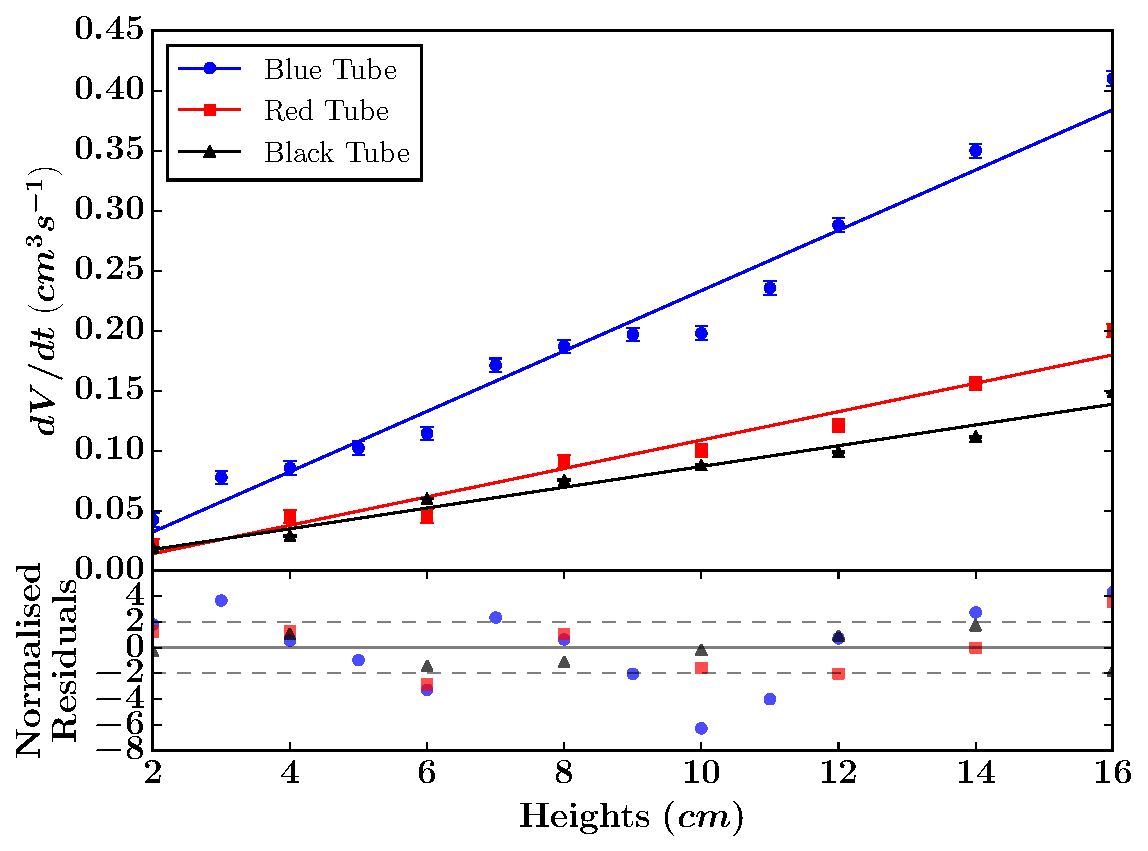
\includegraphics[width=9cm]{fig1-3}
\caption[]{The volume flow rate of water ($dV/dt$) as a function of height ($h$) for three capillary tubes of different diameter. The vertical error bars on $dV/dt$ are too small to be seen.}
\label{fig:fig2}
\end{center}
\end{figure}

\squeezeup
\squeezeup
\squeezeup

\begin{table}[h!]
\centering
\begin{tabular}{ |c|c|c|c| } 
 \hline
 \textbf{Tube} & \textbf{Radius, a [mm]} & \textbf{$\boldsymbol{\eta_{water}}$ [mPa {s}]} & \textbf{$\boldsymbol{\chi^2_{\nu}}$} \\ [0.5ex] 
 \hline
 $Blue$ &$0.55\pm0.03$ & $1.0\pm0.2$ & 11.0 \\ 
 $Red$ & $0.47\pm0.03$ & $1.1\pm0.3$ & 5.31 \\
 $Black$ & $0.46\pm0.03$ & $1.0\pm0.3$ & 1.94 \\
 
 \hline
\end{tabular}
\caption{Radius of the three tubes, their respective calculated value for $\eta_{water}$, and the reduced chi-squared statistic, $\chi^2$, is shown for each tube as well.}
\label{table:1}
\end{table}

\squeezeup
\squeezeup

\vspace{-3ex}
\section{Discussion}
\vspace{-2ex}
From an initial inspection of Fig. \ref{fig:fig2} we see that the change in $dV/dt$ with $h$ appears to follow a linear regression model. However, the normalised residuals are not contained within $\pm 2$, for the blue tube about 46\% of the points are outside this. This suggests that the fit of the blue data is not good and further experimentation may be required. 

We can further explore the validity of our data by looking at the calculated reduced chi-squared statistics. A reasonable fit to the model should expect $\chi^2_{\nu}$ to be approximately one \cite{hughesandhayes}. After minimising and reducing $\chi^2$ using 'Solver' on Excel, we see that the black tube has the closest $\chi^2_{\nu}$ value to unity, so we can say this set of data has the best fit to the linear model, and that the viscosity value calculated here would be the most acceptable. [[?]] This could be because the black tube had the smallest diameter so the flow rate would be slower, thus the actual volume that flowed out would be easier to measure.

From Table \ref{table:1} we can see that all three values of $\eta$ do agree with each other within their experimental errors. Although, the calculated value for the viscosity using the blue tube has the biggest disparity when compared with the literature value, it also has the greatest $\chi^2_{\nu}$ value. The data not fitting the model could be due to the volume that was measured, was not the exact value that had flowed out. With increased flow rate from greater diameter, it proved more difficult to know when exactly to stop the flow. 

Going back to the black tube 

With our experimentation, there were other limitations affecting the measured value for the volume of water. It is highly likely that the $V$ we measured was not the actual value that had flowed out of the tank for each tube. This problem arose due to the fact that there was always some water left within the pipette when transferring from beaker to the measuring cylinder, and also that the capillary tube would not form a perfectly air tight seal with the tank so water inevitably leaked out.

Another experimental limitation was that the diameter of each tube was not uniform throughout. With this, we see that due to the tapering of the tube, the volume flow rate would have been reduced as the flow of the water would have been non-uniform. Thus again, shifting our measured quantities from their true values.

With our analysis, other factors were not taken into account during our calculations such as the variation in the density of water with temperature change. From the Thiesen-Scheel-Diesselhorst equation \cite{dentemp}, we see that as the temperature of water increases, the density decreases, meaning that the viscosity will decrease as a result. While we assumed that the fluid was incompressible, our calculations could be altered to account for this and thus potentially produce a result for $\eta_{water}$ which would closer to the literature value.

For our experiment we took only one set of data for each tube as we were constrained by time. In future experiments it would be highly beneficial to take repeat data sets for each tube. This would allow us to create a clearer picture of whether or not our data is a good fit to the model, and if our viscosities truly disagree with the stated literature value. 

\vspace{-5ex}
\section{Conclusions}
\vspace{-2ex}
 
In conclusion, from measurements of the volume and mass of water, it was possible to calculate an average value for the viscosity of water. This was found to be $1.00 \pm 0.03$ mPa s, which is not consistent with the literature value of $1.679$  mPa {s} \cite{crc}. Our data did not prove to be a perfect fit to the linear regression model, and more experimentation would be required to produce stronger [[?]] outcomes?
\squeezeup
\squeezeup

\begin{thebibliography}{5}
\bibitem{poiseuillehagen}
	Salvatore P. Sutera and Richard Skalak
	\textit{The History of Poiseuille's Law}.
	Annu. Rev. Fluid Mech., 1993.
	
\bibitem{collegephysics}
	Raymond A. Serway, Chris Vuille, and Jerry S. Faughin
	\textit{College Physics, 8th Edition}.
	Brooks/Cole, Belmont, CA, USA, 2009.

\bibitem{youngandfreedman} 
	Hugh D. Young and Roger A. Freedman.
	\textit{University Physics with Modern Physics, 13th Edition}. 
	Pearson Education Limited, Essex, UK, 2015.
	
\bibitem{crc} 
	W. M. Haynes.
	\textit{CRC Handbook of Chemistry and Physics, 92nd Edition}. 
	CRC Press, Florida, USA, 2011.
	
\bibitem{dentemp} 
	J. L. Martin and S. C. McCutcheon
	\textit{Hydrodynamics and Transport for Water Quality Modelling}. 
	CRC Press, Florida, USA, 1999.
	
\bibitem{hughesandhayes} 
	I. G. Hughes and T. P. A. Hase
	\textit{Measurements and their Uncertainties}. 
	Oxford University Press, Oxford, UK, 2010.
	
\end{thebibliography}
\clearpage

\vfill
\twocolumngrid
\vspace{-3ex}
\section*{Appendix}
\vspace{-2ex}

For the data that was collected using analogue devices, the precision is half a devision \cite{crc}. The uncertainty in the measurement of the height $h$ vertically up the side of the water tank was found to be $0.5$ cm. The volume of water within the measuring cylinder was $0.5$ cm$^{3}$. [[? how these uncertainties arise -> the markings on the side and stuff]] 

With the capillary tubes while a $30$ cm was used to measure the length of the tube, and that respective error was $0.5$ cm. However, the diameter of the tube was measured using a travelling microscope setup, with the measurements read off a vernier scale. We found that we could not say the uncertainty was $0.0001$ cm as there was uncertainty in the parallax of where we defined the beginning and end of the diameter, and whether or not we could tell which tick marks lined up on the vernier scale. So instead, we took the uncertainty on the diameter, and subsequently the radius [[????]] to be $0.0003$ cm. 

For the measured mass, the uncertainty 

\clearpage
\end{document}